\documentclass[twoside]{book}

% Packages required by doxygen
\usepackage{fixltx2e}
\usepackage{calc}
\usepackage{doxygen}
\usepackage[export]{adjustbox} % also loads graphicx
\usepackage{graphicx}
\usepackage[utf8]{inputenc}
\usepackage{makeidx}
\usepackage{multicol}
\usepackage{multirow}
\PassOptionsToPackage{warn}{textcomp}
\usepackage{textcomp}
\usepackage[nointegrals]{wasysym}
\usepackage[table]{xcolor}

% Font selection
\usepackage[T1]{fontenc}
\usepackage[scaled=.90]{helvet}
\usepackage{courier}
\usepackage{amssymb}
\usepackage{sectsty}
\renewcommand{\familydefault}{\sfdefault}
\allsectionsfont{%
  \fontseries{bc}\selectfont%
  \color{darkgray}%
}
\renewcommand{\DoxyLabelFont}{%
  \fontseries{bc}\selectfont%
  \color{darkgray}%
}
\newcommand{\+}{\discretionary{\mbox{\scriptsize$\hookleftarrow$}}{}{}}

% Page & text layout
\usepackage{geometry}
\geometry{%
  a4paper,%
  top=2.5cm,%
  bottom=2.5cm,%
  left=2.5cm,%
  right=2.5cm%
}
\tolerance=750
\hfuzz=15pt
\hbadness=750
\setlength{\emergencystretch}{15pt}
\setlength{\parindent}{0cm}
\setlength{\parskip}{0.2cm}
\makeatletter
\renewcommand{\paragraph}{%
  \@startsection{paragraph}{4}{0ex}{-1.0ex}{1.0ex}{%
    \normalfont\normalsize\bfseries\SS@parafont%
  }%
}
\renewcommand{\subparagraph}{%
  \@startsection{subparagraph}{5}{0ex}{-1.0ex}{1.0ex}{%
    \normalfont\normalsize\bfseries\SS@subparafont%
  }%
}
\makeatother

% Headers & footers
\usepackage{fancyhdr}
\pagestyle{fancyplain}
\fancyhead[LE]{\fancyplain{}{\bfseries\thepage}}
\fancyhead[CE]{\fancyplain{}{}}
\fancyhead[RE]{\fancyplain{}{\bfseries\leftmark}}
\fancyhead[LO]{\fancyplain{}{\bfseries\rightmark}}
\fancyhead[CO]{\fancyplain{}{}}
\fancyhead[RO]{\fancyplain{}{\bfseries\thepage}}
\fancyfoot[LE]{\fancyplain{}{}}
\fancyfoot[CE]{\fancyplain{}{}}
\fancyfoot[RE]{\fancyplain{}{\bfseries\scriptsize Generated on Sun Dec 6 2015 16\+:03\+:51 for Buff\+Life by Doxygen }}
\fancyfoot[LO]{\fancyplain{}{\bfseries\scriptsize Generated on Sun Dec 6 2015 16\+:03\+:51 for Buff\+Life by Doxygen }}
\fancyfoot[CO]{\fancyplain{}{}}
\fancyfoot[RO]{\fancyplain{}{}}
\renewcommand{\footrulewidth}{0.4pt}
\renewcommand{\chaptermark}[1]{%
  \markboth{#1}{}%
}
\renewcommand{\sectionmark}[1]{%
  \markright{\thesection\ #1}%
}

% Indices & bibliography
\usepackage{natbib}
\usepackage[titles]{tocloft}
\setcounter{tocdepth}{3}
\setcounter{secnumdepth}{5}
\makeindex

% Hyperlinks (required, but should be loaded last)
\usepackage{ifpdf}
\ifpdf
  \usepackage[pdftex,pagebackref=true]{hyperref}
\else
  \usepackage[ps2pdf,pagebackref=true]{hyperref}
\fi
\hypersetup{%
  colorlinks=true,%
  linkcolor=blue,%
  citecolor=blue,%
  unicode%
}

% Custom commands
\newcommand{\clearemptydoublepage}{%
  \newpage{\pagestyle{empty}\cleardoublepage}%
}


%===== C O N T E N T S =====

\begin{document}

% Titlepage & ToC
\hypersetup{pageanchor=false,
             bookmarks=true,
             bookmarksnumbered=true,
             pdfencoding=unicode
            }
\pagenumbering{roman}
\begin{titlepage}
\vspace*{7cm}
\begin{center}%
{\Large Buff\+Life }\\
\vspace*{1cm}
{\large Generated by Doxygen 1.8.10}\\
\vspace*{0.5cm}
{\small Sun Dec 6 2015 16:03:51}\\
\end{center}
\end{titlepage}
\clearemptydoublepage
\tableofcontents
\clearemptydoublepage
\pagenumbering{arabic}
\hypersetup{pageanchor=true}

%--- Begin generated contents ---
\chapter{Hierarchical Index}
\section{Class Hierarchy}
This inheritance list is sorted roughly, but not completely, alphabetically\+:\begin{DoxyCompactList}
\item Activity\begin{DoxyCompactList}
\item \contentsline{section}{com.\+bufflife.\+bufflife.\+bus\+Tracker}{\pageref{classcom_1_1bufflife_1_1bufflife_1_1bus_tracker}}{}
\item \contentsline{section}{com.\+bufflife.\+bufflife.\+campus\+Alerts}{\pageref{classcom_1_1bufflife_1_1bufflife_1_1campus_alerts}}{}
\item \contentsline{section}{com.\+bufflife.\+bufflife.\+culogin}{\pageref{classcom_1_1bufflife_1_1bufflife_1_1culogin}}{}
\item \contentsline{section}{com.\+bufflife.\+bufflife.\+dining\+Hall\+Menu}{\pageref{classcom_1_1bufflife_1_1bufflife_1_1dining_hall_menu}}{}
\item \contentsline{section}{com.\+bufflife.\+bufflife.\+map\+View}{\pageref{classcom_1_1bufflife_1_1bufflife_1_1map_view}}{}
\end{DoxyCompactList}
\item App\+Compat\+Activity\begin{DoxyCompactList}
\item \contentsline{section}{com.\+bufflife.\+bufflife.\+Main\+Activity}{\pageref{classcom_1_1bufflife_1_1bufflife_1_1_main_activity}}{}
\end{DoxyCompactList}
\item Async\+Task\begin{DoxyCompactList}
\item \contentsline{section}{com.\+bufflife.\+bufflife.\+dining\+Hall\+Menu.\+dining\+Hall\+Menu\+Background}{\pageref{classcom_1_1bufflife_1_1bufflife_1_1dining_hall_menu_1_1dining_hall_menu_background}}{}
\end{DoxyCompactList}
\end{DoxyCompactList}

\chapter{Class Index}
\section{Class List}
Here are the classes, structs, unions and interfaces with brief descriptions\+:\begin{DoxyCompactList}
\item\contentsline{section}{\hyperlink{classcom_1_1bufflife_1_1bufflife_1_1bus_tracker}{com.\+bufflife.\+bufflife.\+bus\+Tracker} }{\pageref{classcom_1_1bufflife_1_1bufflife_1_1bus_tracker}}{}
\item\contentsline{section}{\hyperlink{classcom_1_1bufflife_1_1bufflife_1_1campus_alerts}{com.\+bufflife.\+bufflife.\+campus\+Alerts} }{\pageref{classcom_1_1bufflife_1_1bufflife_1_1campus_alerts}}{}
\item\contentsline{section}{\hyperlink{classcom_1_1bufflife_1_1bufflife_1_1culogin}{com.\+bufflife.\+bufflife.\+culogin} }{\pageref{classcom_1_1bufflife_1_1bufflife_1_1culogin}}{}
\item\contentsline{section}{\hyperlink{classcom_1_1bufflife_1_1bufflife_1_1dining_hall_menu}{com.\+bufflife.\+bufflife.\+dining\+Hall\+Menu} }{\pageref{classcom_1_1bufflife_1_1bufflife_1_1dining_hall_menu}}{}
\item\contentsline{section}{\hyperlink{classcom_1_1bufflife_1_1bufflife_1_1dining_hall_menu_1_1dining_hall_menu_background}{com.\+bufflife.\+bufflife.\+dining\+Hall\+Menu.\+dining\+Hall\+Menu\+Background} }{\pageref{classcom_1_1bufflife_1_1bufflife_1_1dining_hall_menu_1_1dining_hall_menu_background}}{}
\item\contentsline{section}{\hyperlink{classcom_1_1bufflife_1_1bufflife_1_1_main_activity}{com.\+bufflife.\+bufflife.\+Main\+Activity} }{\pageref{classcom_1_1bufflife_1_1bufflife_1_1_main_activity}}{}
\item\contentsline{section}{\hyperlink{classcom_1_1bufflife_1_1bufflife_1_1map_view}{com.\+bufflife.\+bufflife.\+map\+View} }{\pageref{classcom_1_1bufflife_1_1bufflife_1_1map_view}}{}
\end{DoxyCompactList}

\chapter{Class Documentation}
\hypertarget{classcom_1_1bufflife_1_1bufflife_1_1bus_tracker}{}\section{com.\+bufflife.\+bufflife.\+bus\+Tracker Class Reference}
\label{classcom_1_1bufflife_1_1bufflife_1_1bus_tracker}\index{com.\+bufflife.\+bufflife.\+bus\+Tracker@{com.\+bufflife.\+bufflife.\+bus\+Tracker}}
Inheritance diagram for com.\+bufflife.\+bufflife.\+bus\+Tracker\+:\begin{figure}[H]
\begin{center}
\leavevmode
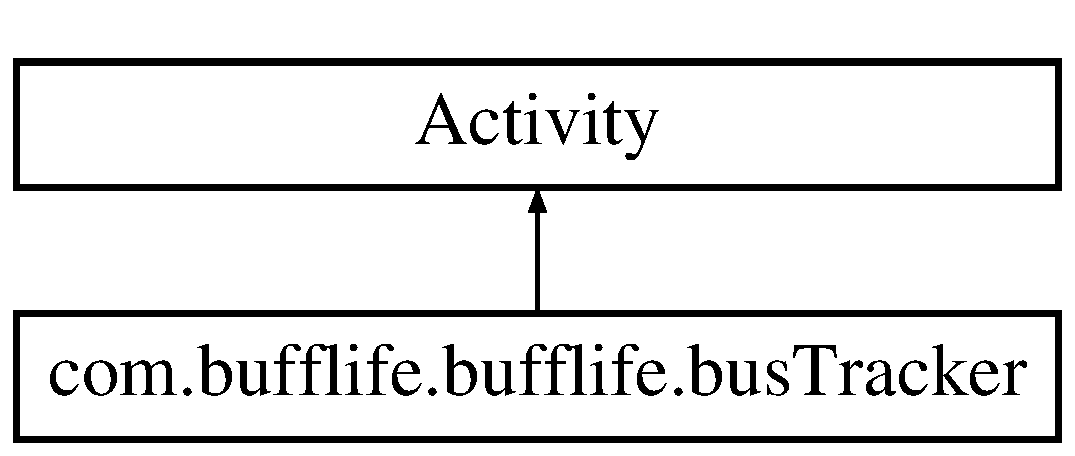
\includegraphics[height=2.000000cm]{classcom_1_1bufflife_1_1bufflife_1_1bus_tracker}
\end{center}
\end{figure}
\subsection*{Public Member Functions}
\begin{DoxyCompactItemize}
\item 
void \hyperlink{classcom_1_1bufflife_1_1bufflife_1_1bus_tracker_ac74ed6517a7e560d1c0788ef53e9688f}{on\+Create} (Bundle saved\+Instance\+State)
\end{DoxyCompactItemize}


\subsection{Detailed Description}
\begin{DoxyAuthor}{Author}
Jesse Bird 
\end{DoxyAuthor}
\begin{DoxyVersion}{Version}
1.\+0 
\end{DoxyVersion}


\subsection{Member Function Documentation}
\hypertarget{classcom_1_1bufflife_1_1bufflife_1_1bus_tracker_ac74ed6517a7e560d1c0788ef53e9688f}{}\index{com\+::bufflife\+::bufflife\+::bus\+Tracker@{com\+::bufflife\+::bufflife\+::bus\+Tracker}!on\+Create@{on\+Create}}
\index{on\+Create@{on\+Create}!com\+::bufflife\+::bufflife\+::bus\+Tracker@{com\+::bufflife\+::bufflife\+::bus\+Tracker}}
\subsubsection[{on\+Create(\+Bundle saved\+Instance\+State)}]{\setlength{\rightskip}{0pt plus 5cm}void com.\+bufflife.\+bufflife.\+bus\+Tracker.\+on\+Create (
\begin{DoxyParamCaption}
\item[{Bundle}]{saved\+Instance\+State}
\end{DoxyParamCaption}
)\hspace{0.3cm}{\ttfamily [inline]}}\label{classcom_1_1bufflife_1_1bufflife_1_1bus_tracker_ac74ed6517a7e560d1c0788ef53e9688f}
Create webview for buffbusmobile.\+etaspot.\+net 
\begin{DoxyParams}{Parameters}
{\em saved\+Instance\+State} & display webview of url within app \\
\hline
\end{DoxyParams}


The documentation for this class was generated from the following file\+:\begin{DoxyCompactItemize}
\item 
bus\+Tracker.\+java\end{DoxyCompactItemize}

\hypertarget{classcom_1_1bufflife_1_1bufflife_1_1campus_alerts}{}\section{com.\+bufflife.\+bufflife.\+campus\+Alerts Class Reference}
\label{classcom_1_1bufflife_1_1bufflife_1_1campus_alerts}\index{com.\+bufflife.\+bufflife.\+campus\+Alerts@{com.\+bufflife.\+bufflife.\+campus\+Alerts}}
Inheritance diagram for com.\+bufflife.\+bufflife.\+campus\+Alerts\+:\begin{figure}[H]
\begin{center}
\leavevmode
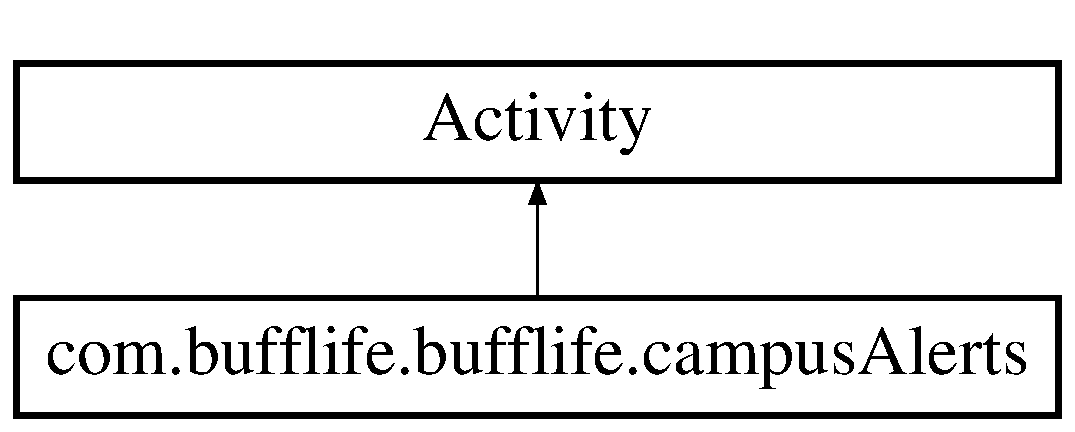
\includegraphics[height=2.000000cm]{classcom_1_1bufflife_1_1bufflife_1_1campus_alerts}
\end{center}
\end{figure}
\subsection*{Public Member Functions}
\begin{DoxyCompactItemize}
\item 
void \hyperlink{classcom_1_1bufflife_1_1bufflife_1_1campus_alerts_af633a15fc57680bdf2f54b05bfefd131}{on\+Create} (Bundle saved\+Instance\+State)
\end{DoxyCompactItemize}


\subsection{Detailed Description}
\begin{DoxyAuthor}{Author}
Jesse Bird 
\end{DoxyAuthor}
\begin{DoxyVersion}{Version}
1.\+0 
\end{DoxyVersion}


\subsection{Member Function Documentation}
\hypertarget{classcom_1_1bufflife_1_1bufflife_1_1campus_alerts_af633a15fc57680bdf2f54b05bfefd131}{}\index{com\+::bufflife\+::bufflife\+::campus\+Alerts@{com\+::bufflife\+::bufflife\+::campus\+Alerts}!on\+Create@{on\+Create}}
\index{on\+Create@{on\+Create}!com\+::bufflife\+::bufflife\+::campus\+Alerts@{com\+::bufflife\+::bufflife\+::campus\+Alerts}}
\subsubsection[{on\+Create(\+Bundle saved\+Instance\+State)}]{\setlength{\rightskip}{0pt plus 5cm}void com.\+bufflife.\+bufflife.\+campus\+Alerts.\+on\+Create (
\begin{DoxyParamCaption}
\item[{Bundle}]{saved\+Instance\+State}
\end{DoxyParamCaption}
)\hspace{0.3cm}{\ttfamily [inline]}}\label{classcom_1_1bufflife_1_1bufflife_1_1campus_alerts_af633a15fc57680bdf2f54b05bfefd131}
Create Webview for twitter alerts 
\begin{DoxyParams}{Parameters}
{\em saved\+Instance\+State} & display webview of url A\+P\+I Still needs to be implented currently goes to external browser since twitter A\+P\+I difficulties \\
\hline
\end{DoxyParams}


The documentation for this class was generated from the following file\+:\begin{DoxyCompactItemize}
\item 
campus\+Alerts.\+java\end{DoxyCompactItemize}

\hypertarget{classcom_1_1bufflife_1_1bufflife_1_1culogin}{}\section{com.\+bufflife.\+bufflife.\+culogin Class Reference}
\label{classcom_1_1bufflife_1_1bufflife_1_1culogin}\index{com.\+bufflife.\+bufflife.\+culogin@{com.\+bufflife.\+bufflife.\+culogin}}
Inheritance diagram for com.\+bufflife.\+bufflife.\+culogin\+:\begin{figure}[H]
\begin{center}
\leavevmode
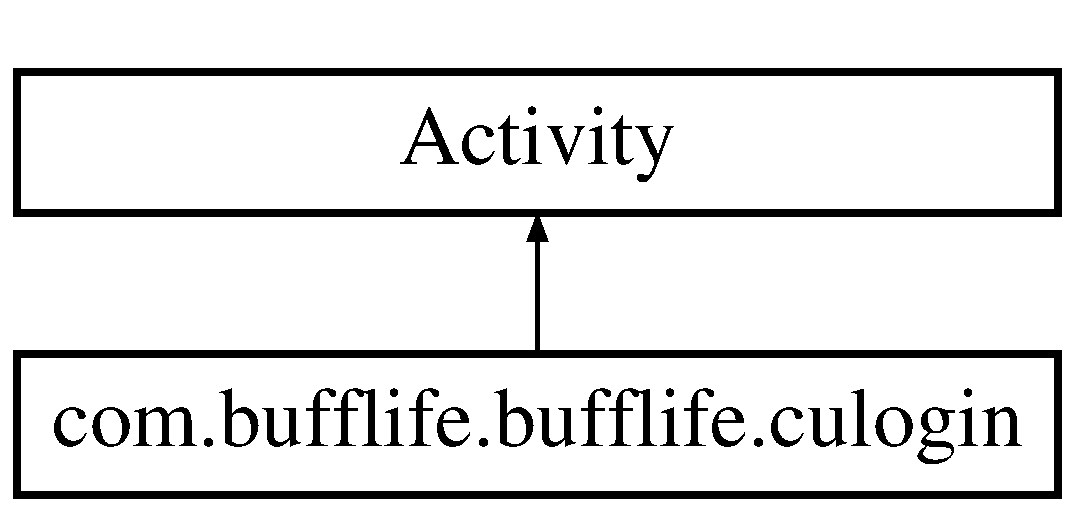
\includegraphics[height=2.000000cm]{classcom_1_1bufflife_1_1bufflife_1_1culogin}
\end{center}
\end{figure}
\subsection*{Classes}
\begin{DoxyCompactItemize}
\item 
class {\bfseries Uri\+Chrome\+Client}
\end{DoxyCompactItemize}
\subsection*{Protected Member Functions}
\begin{DoxyCompactItemize}
\item 
void \hyperlink{classcom_1_1bufflife_1_1bufflife_1_1culogin_a68f2776af67107d724abb1341a70bcb4}{on\+Create} (Bundle saved\+Instance\+State)
\end{DoxyCompactItemize}


\subsection{Member Function Documentation}
\hypertarget{classcom_1_1bufflife_1_1bufflife_1_1culogin_a68f2776af67107d724abb1341a70bcb4}{}\index{com\+::bufflife\+::bufflife\+::culogin@{com\+::bufflife\+::bufflife\+::culogin}!on\+Create@{on\+Create}}
\index{on\+Create@{on\+Create}!com\+::bufflife\+::bufflife\+::culogin@{com\+::bufflife\+::bufflife\+::culogin}}
\subsubsection[{on\+Create(\+Bundle saved\+Instance\+State)}]{\setlength{\rightskip}{0pt plus 5cm}void com.\+bufflife.\+bufflife.\+culogin.\+on\+Create (
\begin{DoxyParamCaption}
\item[{Bundle}]{saved\+Instance\+State}
\end{DoxyParamCaption}
)\hspace{0.3cm}{\ttfamily [inline]}, {\ttfamily [protected]}}\label{classcom_1_1bufflife_1_1bufflife_1_1culogin_a68f2776af67107d724abb1341a70bcb4}
Creating web A\+P\+I with webview 
\begin{DoxyParams}{Parameters}
{\em saved\+Instance\+State} & display within app \\
\hline
\end{DoxyParams}


The documentation for this class was generated from the following file\+:\begin{DoxyCompactItemize}
\item 
culogin.\+java\end{DoxyCompactItemize}

\hypertarget{classcom_1_1bufflife_1_1bufflife_1_1dining_hall_menu}{}\section{com.\+bufflife.\+bufflife.\+dining\+Hall\+Menu Class Reference}
\label{classcom_1_1bufflife_1_1bufflife_1_1dining_hall_menu}\index{com.\+bufflife.\+bufflife.\+dining\+Hall\+Menu@{com.\+bufflife.\+bufflife.\+dining\+Hall\+Menu}}
Inheritance diagram for com.\+bufflife.\+bufflife.\+dining\+Hall\+Menu\+:\begin{figure}[H]
\begin{center}
\leavevmode
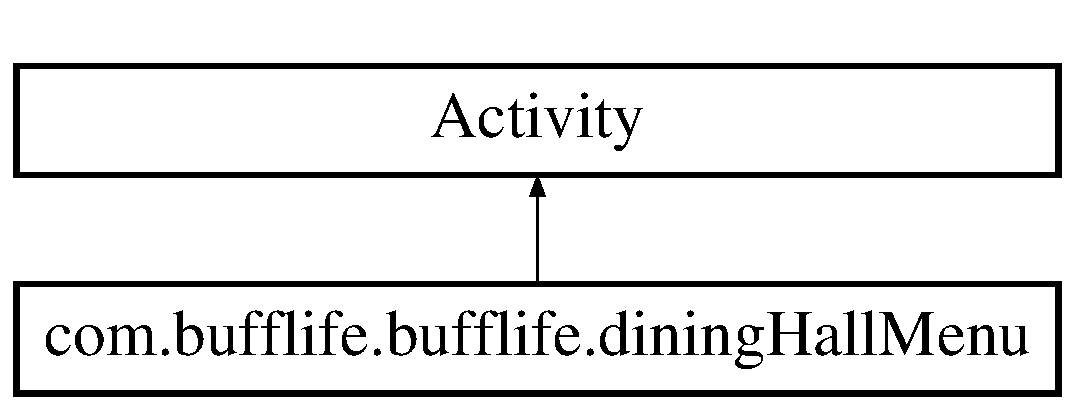
\includegraphics[height=2.000000cm]{classcom_1_1bufflife_1_1bufflife_1_1dining_hall_menu}
\end{center}
\end{figure}
\subsection*{Classes}
\begin{DoxyCompactItemize}
\item 
class \hyperlink{classcom_1_1bufflife_1_1bufflife_1_1dining_hall_menu_1_1dining_hall_menu_background}{dining\+Hall\+Menu\+Background}
\end{DoxyCompactItemize}
\subsection*{Public Member Functions}
\begin{DoxyCompactItemize}
\item 
\hypertarget{classcom_1_1bufflife_1_1bufflife_1_1dining_hall_menu_a62abbdded56c5e036a17639715919840}{}void {\bfseries on\+Create} (Bundle saved\+Instance\+State)\label{classcom_1_1bufflife_1_1bufflife_1_1dining_hall_menu_a62abbdded56c5e036a17639715919840}

\end{DoxyCompactItemize}


\subsection{Detailed Description}
$<$$<$$<$$<$$<$$<$$<$ Updated upstream \begin{DoxyAuthor}{Author}
Created by danielyedidovich on 11/11/15. 

last edited by Kyle Knight 11/18/2015 had to change to async task to work We could also simplify to only show meals based on time of day but I think it makes more sense to see the whole week. \subsection*{Also my I\textquotesingle{}m only getting a saturday value for the calendar date and it is definitely not saturday... }

Created by danielyedidovich \begin{quote}
\begin{quote}
\begin{quote}
\begin{quote}
\begin{quote}
\begin{quote}
\begin{quote}
Stashed changes\end{quote}
\end{quote}
\end{quote}
\end{quote}
\end{quote}
\end{quote}
\end{quote}

\end{DoxyAuthor}


The documentation for this class was generated from the following file\+:\begin{DoxyCompactItemize}
\item 
dining\+Hall\+Menu.\+java\end{DoxyCompactItemize}

\hypertarget{classcom_1_1bufflife_1_1bufflife_1_1dining_hall_menu_1_1dining_hall_menu_background}{}\section{com.\+bufflife.\+bufflife.\+dining\+Hall\+Menu.\+dining\+Hall\+Menu\+Background Class Reference}
\label{classcom_1_1bufflife_1_1bufflife_1_1dining_hall_menu_1_1dining_hall_menu_background}\index{com.\+bufflife.\+bufflife.\+dining\+Hall\+Menu.\+dining\+Hall\+Menu\+Background@{com.\+bufflife.\+bufflife.\+dining\+Hall\+Menu.\+dining\+Hall\+Menu\+Background}}
Inheritance diagram for com.\+bufflife.\+bufflife.\+dining\+Hall\+Menu.\+dining\+Hall\+Menu\+Background\+:\begin{figure}[H]
\begin{center}
\leavevmode
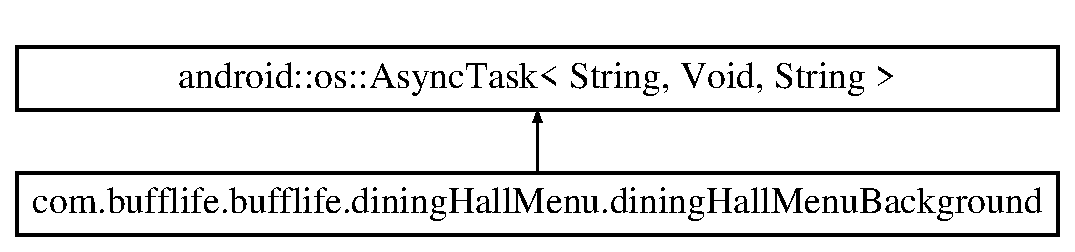
\includegraphics[height=2.000000cm]{classcom_1_1bufflife_1_1bufflife_1_1dining_hall_menu_1_1dining_hall_menu_background}
\end{center}
\end{figure}
\subsection*{Public Member Functions}
\begin{DoxyCompactItemize}
\item 
\hypertarget{classcom_1_1bufflife_1_1bufflife_1_1dining_hall_menu_1_1dining_hall_menu_background_a8ca54a70ad2ce79cd4b4bc9f8e69d123}{}String {\bfseries do\+In\+Background} (String...\+strings)\label{classcom_1_1bufflife_1_1bufflife_1_1dining_hall_menu_1_1dining_hall_menu_background_a8ca54a70ad2ce79cd4b4bc9f8e69d123}

\end{DoxyCompactItemize}
\subsection*{Protected Member Functions}
\begin{DoxyCompactItemize}
\item 
\hypertarget{classcom_1_1bufflife_1_1bufflife_1_1dining_hall_menu_1_1dining_hall_menu_background_a5176926158f2f9691b9aff4a2212e502}{}void {\bfseries on\+Post\+Execute} (String s)\label{classcom_1_1bufflife_1_1bufflife_1_1dining_hall_menu_1_1dining_hall_menu_background_a5176926158f2f9691b9aff4a2212e502}

\end{DoxyCompactItemize}


\subsection{Detailed Description}
\begin{DoxyAuthor}{Author}
Created by Kyle on 11/12/2015. 
\end{DoxyAuthor}


The documentation for this class was generated from the following file\+:\begin{DoxyCompactItemize}
\item 
dining\+Hall\+Menu.\+java\end{DoxyCompactItemize}

\hypertarget{classcom_1_1bufflife_1_1bufflife_1_1_main_activity}{}\section{com.\+bufflife.\+bufflife.\+Main\+Activity Class Reference}
\label{classcom_1_1bufflife_1_1bufflife_1_1_main_activity}\index{com.\+bufflife.\+bufflife.\+Main\+Activity@{com.\+bufflife.\+bufflife.\+Main\+Activity}}
Inheritance diagram for com.\+bufflife.\+bufflife.\+Main\+Activity\+:\begin{figure}[H]
\begin{center}
\leavevmode
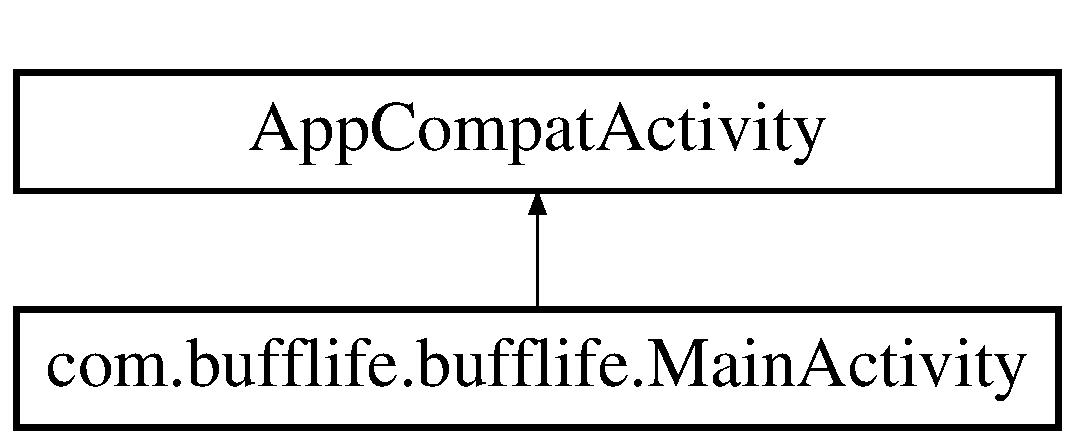
\includegraphics[height=2.000000cm]{classcom_1_1bufflife_1_1bufflife_1_1_main_activity}
\end{center}
\end{figure}
\subsection*{Public Member Functions}
\begin{DoxyCompactItemize}
\item 
boolean \hyperlink{classcom_1_1bufflife_1_1bufflife_1_1_main_activity_a8970eccd15a081a309a3557e442789f1}{on\+Create\+Options\+Menu} (Menu menu)
\end{DoxyCompactItemize}
\subsection*{Public Attributes}
\begin{DoxyCompactItemize}
\item 
\hypertarget{classcom_1_1bufflife_1_1bufflife_1_1_main_activity_ad63e0a8ab197f64591d22da45ce3e778}{}Button {\bfseries buttonmap\+View}\label{classcom_1_1bufflife_1_1bufflife_1_1_main_activity_ad63e0a8ab197f64591d22da45ce3e778}

\item 
\hypertarget{classcom_1_1bufflife_1_1bufflife_1_1_main_activity_a74e38f5103079101807345c98ba6b0db}{}Button {\bfseries buttonbus\+Tracker}\label{classcom_1_1bufflife_1_1bufflife_1_1_main_activity_a74e38f5103079101807345c98ba6b0db}

\item 
\hypertarget{classcom_1_1bufflife_1_1bufflife_1_1_main_activity_a038f64ee4f3113d798219aa8a305bb3f}{}Button {\bfseries buttoncampus\+Alerts}\label{classcom_1_1bufflife_1_1bufflife_1_1_main_activity_a038f64ee4f3113d798219aa8a305bb3f}

\item 
\hypertarget{classcom_1_1bufflife_1_1bufflife_1_1_main_activity_a495968a469e7ddbc41a004c4aae72a9f}{}Button {\bfseries buttonculogin}\label{classcom_1_1bufflife_1_1bufflife_1_1_main_activity_a495968a469e7ddbc41a004c4aae72a9f}

\item 
\hypertarget{classcom_1_1bufflife_1_1bufflife_1_1_main_activity_a6977b7ad5893e52140bea50c46d7dfbb}{}Button {\bfseries buttondining\+Hall\+Menu}\label{classcom_1_1bufflife_1_1bufflife_1_1_main_activity_a6977b7ad5893e52140bea50c46d7dfbb}

\end{DoxyCompactItemize}
\subsection*{Protected Member Functions}
\begin{DoxyCompactItemize}
\item 
void \hyperlink{classcom_1_1bufflife_1_1bufflife_1_1_main_activity_a287ff6c199dd2f0c8335cae6951b3c98}{on\+Create} (Bundle saved\+Instance\+State)
\end{DoxyCompactItemize}


\subsection{Member Function Documentation}
\hypertarget{classcom_1_1bufflife_1_1bufflife_1_1_main_activity_a287ff6c199dd2f0c8335cae6951b3c98}{}\index{com\+::bufflife\+::bufflife\+::\+Main\+Activity@{com\+::bufflife\+::bufflife\+::\+Main\+Activity}!on\+Create@{on\+Create}}
\index{on\+Create@{on\+Create}!com\+::bufflife\+::bufflife\+::\+Main\+Activity@{com\+::bufflife\+::bufflife\+::\+Main\+Activity}}
\subsubsection[{on\+Create(\+Bundle saved\+Instance\+State)}]{\setlength{\rightskip}{0pt plus 5cm}void com.\+bufflife.\+bufflife.\+Main\+Activity.\+on\+Create (
\begin{DoxyParamCaption}
\item[{Bundle}]{saved\+Instance\+State}
\end{DoxyParamCaption}
)\hspace{0.3cm}{\ttfamily [inline]}, {\ttfamily [protected]}}\label{classcom_1_1bufflife_1_1bufflife_1_1_main_activity_a287ff6c199dd2f0c8335cae6951b3c98}
Creating all buttons 
\begin{DoxyParams}{Parameters}
{\em saved\+Instance\+State} & \\
\hline
\end{DoxyParams}
Button to go to \hyperlink{classcom_1_1bufflife_1_1bufflife_1_1map_view}{map\+View} class 
\begin{DoxyParams}{Parameters}
{\em v} & \\
\hline
\end{DoxyParams}
Button to go to \hyperlink{classcom_1_1bufflife_1_1bufflife_1_1bus_tracker}{bus\+Tracker} class 
\begin{DoxyParams}{Parameters}
{\em v} & On click go the view\\
\hline
\end{DoxyParams}
Button to go to \hyperlink{classcom_1_1bufflife_1_1bufflife_1_1campus_alerts}{campus\+Alerts} class 
\begin{DoxyParams}{Parameters}
{\em v} & On click go the view\\
\hline
\end{DoxyParams}
Button to go to culogin class 
\begin{DoxyParams}{Parameters}
{\em v} & On click go the view\\
\hline
\end{DoxyParams}
Button to go to \hyperlink{classcom_1_1bufflife_1_1bufflife_1_1dining_hall_menu}{dining\+Hall\+Menu} Class 
\begin{DoxyParams}{Parameters}
{\em v} & On click go the view \\
\hline
\end{DoxyParams}
\begin{DoxyAuthor}{Author}
Daniel Yedidovich 
\end{DoxyAuthor}
\begin{DoxyVersion}{Version}
1.\+5
\end{DoxyVersion}
\hypertarget{classcom_1_1bufflife_1_1bufflife_1_1_main_activity_a8970eccd15a081a309a3557e442789f1}{}\index{com\+::bufflife\+::bufflife\+::\+Main\+Activity@{com\+::bufflife\+::bufflife\+::\+Main\+Activity}!on\+Create\+Options\+Menu@{on\+Create\+Options\+Menu}}
\index{on\+Create\+Options\+Menu@{on\+Create\+Options\+Menu}!com\+::bufflife\+::bufflife\+::\+Main\+Activity@{com\+::bufflife\+::bufflife\+::\+Main\+Activity}}
\subsubsection[{on\+Create\+Options\+Menu(\+Menu menu)}]{\setlength{\rightskip}{0pt plus 5cm}boolean com.\+bufflife.\+bufflife.\+Main\+Activity.\+on\+Create\+Options\+Menu (
\begin{DoxyParamCaption}
\item[{Menu}]{menu}
\end{DoxyParamCaption}
)\hspace{0.3cm}{\ttfamily [inline]}}\label{classcom_1_1bufflife_1_1bufflife_1_1_main_activity_a8970eccd15a081a309a3557e442789f1}
Creating the Action Bar 
\begin{DoxyParams}{Parameters}
{\em menu} & to create menu \\
\hline
\end{DoxyParams}
\begin{DoxyReturn}{Returns}
action bar currently not used since no action bar 
\end{DoxyReturn}


The documentation for this class was generated from the following file\+:\begin{DoxyCompactItemize}
\item 
Main\+Activity.\+java\end{DoxyCompactItemize}

\hypertarget{classcom_1_1bufflife_1_1bufflife_1_1map_view}{}\section{com.\+bufflife.\+bufflife.\+map\+View Class Reference}
\label{classcom_1_1bufflife_1_1bufflife_1_1map_view}\index{com.\+bufflife.\+bufflife.\+map\+View@{com.\+bufflife.\+bufflife.\+map\+View}}
Inheritance diagram for com.\+bufflife.\+bufflife.\+map\+View\+:\begin{figure}[H]
\begin{center}
\leavevmode
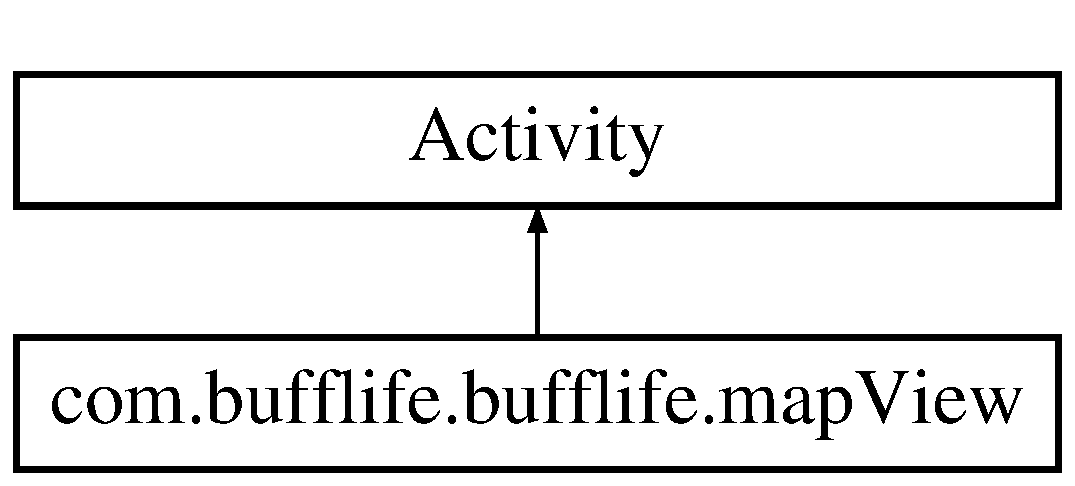
\includegraphics[height=2.000000cm]{classcom_1_1bufflife_1_1bufflife_1_1map_view}
\end{center}
\end{figure}
\subsection*{Public Member Functions}
\begin{DoxyCompactItemize}
\item 
void \hyperlink{classcom_1_1bufflife_1_1bufflife_1_1map_view_a59f93b146f6ea2db381bcaddbecbcde9}{on\+Create} (Bundle saved\+Instance\+State)
\end{DoxyCompactItemize}


\subsection{Member Function Documentation}
\hypertarget{classcom_1_1bufflife_1_1bufflife_1_1map_view_a59f93b146f6ea2db381bcaddbecbcde9}{}\index{com\+::bufflife\+::bufflife\+::map\+View@{com\+::bufflife\+::bufflife\+::map\+View}!on\+Create@{on\+Create}}
\index{on\+Create@{on\+Create}!com\+::bufflife\+::bufflife\+::map\+View@{com\+::bufflife\+::bufflife\+::map\+View}}
\subsubsection[{on\+Create(\+Bundle saved\+Instance\+State)}]{\setlength{\rightskip}{0pt plus 5cm}void com.\+bufflife.\+bufflife.\+map\+View.\+on\+Create (
\begin{DoxyParamCaption}
\item[{Bundle}]{saved\+Instance\+State}
\end{DoxyParamCaption}
)\hspace{0.3cm}{\ttfamily [inline]}}\label{classcom_1_1bufflife_1_1bufflife_1_1map_view_a59f93b146f6ea2db381bcaddbecbcde9}
Creating webview for cubouldermap.\+com 
\begin{DoxyParams}{Parameters}
{\em saved\+Instance\+State} & display webview of url within app \\
\hline
\end{DoxyParams}


The documentation for this class was generated from the following file\+:\begin{DoxyCompactItemize}
\item 
map\+View.\+java\end{DoxyCompactItemize}

%--- End generated contents ---

% Index
\backmatter
\newpage
\phantomsection
\clearemptydoublepage
\addcontentsline{toc}{chapter}{Index}
\printindex

\end{document}
